\documentclass[master=elt,masteroption=eg,dutch,oneside]{kulemt}
\setup{title={DSP-implementatie - Imageprocessing in MATLAB },
  author={Andries Gert-Jan\and Dejager Xavier\and Steen Nick},
  promotor={ing.\ Dries Debouvere},
  %assessor={Ir.\,W. Eetveel\and W. Eetrest},
  assistant={ing.\ Dries Debouvere}}

\setup{font=lm}

\usepackage{graphicx}
\usepackage{titlesec}
\usepackage{listings}
\usepackage{color}
\usepackage{float}


\usepackage{amsmath}


\definecolor{mygreen}{rgb}{0,0.6,0}
\definecolor{mygray}{rgb}{0.5,0.5,0.5}
\definecolor{mymauve}{rgb}{0.58,0,0.82}

\lstset{ %
  backgroundcolor=\color{white},   % choose the background color; you must add \usepackage{color} or \usepackage{xcolor}
  basicstyle=\footnotesize\ttfamily,% the size of the fonts that are used for the code
  breakatwhitespace=false,         % sets if automatic breaks should only happen at whitespace
  breaklines=true,                 % sets automatic line breaking
  captionpos=b,                    % sets the caption-position to bottom
  commentstyle=\color{mygreen},    % comment style
  deletekeywords={...},            % if you want to delete keywords from the given language
  escapeinside={\%*}{*)},          % if you want to add LaTeX within your code
  extendedchars=true,              % lets you use non-ASCII characters; for 8-bits encodings only, does not work with UTF-8
  frame=single,                    % adds a frame around the code
  keepspaces=true,                 % keeps spaces in text, useful for keeping indentation of code (possibly needs columns=flexible)
  keywordstyle=\color{blue},       % keyword style
  language=Matlab,                 % the language of the code
  morekeywords={*,...},            % if you want to add more keywords to the set
  numbers=none,                    % where to put the line-numbers; possible values are (none, left, right)
  numbersep=2pt,                   % how far the line-numbers are from the code
  numberstyle=\tiny\color{mygray}, % the style that is used for the line-numbers
  rulecolor=\color{black},         % if not set, the frame-color may be changed on line-breaks within not-black text (e.g. comments (green here))
  showspaces=false,                % show spaces everywhere adding particular underscores; it overrides 'showstringspaces'
  showstringspaces=false,          % underline spaces within strings only
  showtabs=false,                  % show tabs within strings adding particular underscores
  stepnumber=2,                    % the step between two line-numbers. If it's 1, each line will be numbered
  stringstyle=\color{mymauve},     % string literal style
  tabsize=2,                       % sets default tabsize to 2 spaces
  title=\lstname ,                 % show the filename of files included with \lstinputlisting; also try caption instead of title
  xleftmargin=2em,
  frame=single,
  framexleftmargin=1.5em
}

%%%%%%%%%%%%%


\lstset{language=Matlab}
\setlength\parindent{0pt}
\titlespacing*{\subsection}{0pt}{1.1\baselineskip}{\baselineskip}
\titlespacing*{\section}{0pt}{1.1\baselineskip}{\baselineskip}

%\includeonly{chap-n}
\begin{document}

\tableofcontents*
\listoffiguresandtables
\chapter{Lijst van gebruikte afkortingen}
\section*{Afkortingen}
\begin{flushleft}
  \renewcommand{\arraystretch}{1.1}
  \begin{tabularx}{\textwidth}{@{}p{12mm}X@{}}
    DSP   & Digital Signal Processing \\
    tv   & Televisie \\
	rgb	& Rood Groen Blauw \\
  \end{tabularx}
\end{flushleft}



% Nu begint de eigenlijke tekst
\mainmatter

\chapter{Inleiding}

\section{Doelstelling}
\par Het doel van deze opdracht is om via het Matlab pakket kennis te maken met de basisprincipes van videoprocessing.
Deze kennismaking is de basis van de vervolgopdracht waarbij gebruikt gemaakt wordt van een DSPprocessor om live
videobeelden realtime te bewerken. Een videosignaal bestaat uit verschillende frames. Wanneer men dus een videosignaal
wil bewerken dient men dit frame per frame aan te pakken. Elk frame kan gezien worden als een afbeelding waarop \'e\'en of 
meerdere bewerkingen gebeuren. Aan de hand van het Matlab pakket wordt kennis verworven in DSP-technieken om kleuren in
afbeeldingen te detecteren en veranderen. \bigskip

\par In het eerste deel van deze opdracht is het de bedoeling om aan de hand van het programma Matlab inzicht te verwerven
in het bewerken van afbeeldingen (frames). Nadien zal in het tweede deel hetzelfde principe realtime toegepast worden op 
videobeelden aan de hand van een DSP-processor, namelijk de BlackFin BF-561.

\section {Achtergrond}

\subsection{Chromakey}

\par Chromakey, ook wel kleurwaarde genoemd is een techniek die v\'e\'el gebruikt wordt in de tv- en filmwereld. Tijdens het 
filmen wordt als achtergrond een scherm gebruikt dat een bepaalde effen kleur heeft. Vervolgens wordt via een computer of DSP-processor
deze achtergrond veranderd door een andere achtergrond die afkomstig kan zijn van een andere videobron of afbeelding. De meest gebruikte
kleuren voor deze achtergrond zijn blauw en groen. De reden hiervoor is dat de kleuren blauw en groen het meest verschillen in tint (hue) van
de kleur van de menselijke huid. \bigskip

\par De chromakey techniek wordt al gebruikt sinds de jaren '90 om speciale effecten in films mogelijk te maken. Ook bij het 
weerbericht en het journaal maakt men vaak gebruik van chromakey om extra informatie achter de presentator weer te geven. Het is zowel mogelijk
om live te achtergrond te wijzigen als nadien. \bigskip

\par De chromakey techniek brengt ook een aantal problemen met zich mee. Zo speelt de belichting van de set een belangrijke
rol tijdens het filmen. Het vormen van schaduw op het scherm kan ervoor zorgen dat dit van kleur veranderd, namelijk het wordt
donkerder waardoor het door het bewerkingsporgramma niet meer herkend wordt als de kleur die dient gewijzigd te worden. Een ander
probleem dat zich voordoet is dat te dunne objecten (bewegende haren) moeilijker kunnen worden waargenomen door de computer. Dit kan zorgen
voor een ongewenst effect. Tot slot dient er ook op gelet te worden dat de presentator zijn kleding geen element bevat in de kleur van het 
scherm dat gebruikt wordt. Anders zou dit ook vervangen worden, net als de achtergrond.\bigskip

\par Naast het gebruik chromakey in de achtergrond is het ook mogelijk om in een videofragment een bepaalde kleur te vervangen door een andere
kleur. Deze techniek kan toegepast worden om oude zwart-wit films om te vormen naar een minimalistische kleurenfilm. Dit kan gedaan worden door
aan een bepaalde grijswaarde een bepaalde kleur toe te kennen. Hierbij speelt de belichting en schaduwen vaak een nadelige rol.

\subsection {Matlab}

\par Matlab is een computerprogramma dat het mogelijk maakt om allerhande wiskundige toepassingen te simuleren. Aan de basis hiervan ligt de 
programmeertaal M-code. Via Matlab is het mogelijk om afbeeldingen in te lezen en vervolgens hierop bewerkingen uit te voeren. Vervolgens kan 
de bewerkte afbeelding terug worden weergegeven. 
 \chapter{Resultaten}

\section{Opgave 1}
	\subsection{Doelstelling}
		\par Deze opgave bestaat eruit om de afbeelding van een Smurf zodanig te bewerken dat de blauwe kleur wordt
		veranderd in een gele kleur. Er dient opgemerkt te worden dat de blauwe kleur waaruit de Smurf bestaat niet \'e\'en type
		blauw is, maar bestaat uit verschillende tinten. Om het blauw naar het geel om te vormen moet dus rekening gehouden
		worden met een bepaald bereik wat de kleur betrefd. 		
	\subsection{Werkwijze en resultaat}
		\subsubsection{Eerste aanpak}
			\par Bij de eerste aanpak werd gekozen om alle kleuren die tussen bepaalde grenswaarden vallen te vervangen door
			een gele kleur. De grenswaarden werden vastgesteld door middel van het programma ColorPic. Dit programma maakt het
			mogelijk om aan de hand van een colorpicker de kleur van een bepaalde pixel op het scherm te bepalen. Proefondervindelijk
			werden zo volgende grenzen bepaald: \bigskip
			
				\begin{table}[H]
				\centering
				\begin{tabular}{ccc}
				\hline
				Kleur & Ondergrens & Bovengrens \\ \hline
				Rood  & 0          & 115        \\
				Groen & 100        & 200        \\
				Blauw & 0          & 255        \\ \hline			
				\end{tabular}
				\caption{Grenswaarden voor blauwe kleur}
				\end{table}
			
			\newpage
			\par Om de blauwe kleur naar geel te veranderen werd elke pixel van de afbeelding doorlopen door middel van een for-structuur.
			Elke pixel wordt gecontroleerd of de kleur tussen de grenswaarden valt. Indien dit het geval is wordt de kleur veranderd naar geel.
			Om de kleur van elke pixel te controleren moest afzonderlijk naar de rood-waarde, groen-waarde en blauw-waarde van elke pixel gekeken worden.
			Deze waarden liggen elk tussen een waarde van 0 en 255. Als gele kleur werd gekozen voor het geel dat overeenstemt met rgb-waarde 255,255,0. 
			De Matlabinplementatie is weergegeven in onderstaand codefragment:\bigskip			
			
			\lstinputlisting[caption=Matlab-code \'e\'erste aanpak]{Matlab/Smurf_1.m}
			
			\newpage
			
			\par Het resultaat van deze code is te zien in onderstaande figuur: 
			
				\begin{figure}[H]
				\centering
				
\includegraphics[width=0.95\textwidth]{Images/resultaat_smurf_1.png}
				\caption{Resultaat kleursverandering Smurf: eerste aanpak}
				\label{fig:smurf_eerste_aanpak}
				\end{figure}
			
			\par Er is op te merken dat dit een vrij drastische verandering is. Het blauw bestaat namelijk niet uit \'e\'en type blauw, maar uit een mix van
			verschillende tinten blauw en het wordt vervangen door slechts \'e\'en type geel. Dit vormt geen aangenaam gevoel voor het menselijk ook. Men neemt 
			dit waar als een niet-natuurlijk beeld. Om dit probleem op te lossen, en het eindresultaat er natuurlijker laten uit te zien werd een tweede aanpak 
			aangewend.	
				
		\subsubsection{Tweede aanpak}
			\par Het resultaat van de eerste aanpak was voor het menselijk oog niet zo goed. Om dit te verbeteren werd gekozen om bij de kleursverandering niet voor
			een vaste kleur geel te kiezen, maar om de rgb-waarden van de gele kleur te laten afhangen van de blauwe kleur. Dit wordt gedaan door bij de blauwe kleur
			een bepaalde waarde op te tellen of af te trekken. Om negatieve waarden te vermijden wordt steeds de absolute waarde genomen. Deze waarden werden 
			experimenteel bepaald en leverden volgend resultaat: \noindent
			
					\begin{table}[H]
					\centering
					\begin{tabular}{cc}
					\hline
					Kleur & Offset   	  \\ \hline
					Rood  & 255 (vast)    \\
					Groen & +54           \\
					Blauw & -215          \\ \hline			
					\end{tabular}
					\caption{Ofset voor conversie blauwe kleur naar gele kleur}
					\end{table}
			\newpage
			
			\par Ook hier wordt elke pixel \'e\'en voor \'e\'en overlopen en gecontroleerd of de rgb-waarden binnen de grenswaarden vallen. Indien dit het geval is 
			wordt er bij de huidige waarde van de pixel een ofset bijgeteld zoals is weergegeven in bovenstaande tabel. De Matlab-code van deze aanpak wordt hieronder
			weergegeven: \bigskip
			
			\lstinputlisting[caption=Matlab-code tweede aanpak]{Matlab/Smurf_2.m}
			
			\newpage
			
			\par Het resultaat van deze aanpak is te zien in volgende figuur:
			
				\begin{figure}[H]
				\centering
				
\includegraphics[width=0.95\textwidth]{Images/resultaat_smurf_2.png}
				\caption{Resultaat kleursverandering Smurf: tweede aanpak}
				\label{fig:smurf_tweede_aanpak}
				\end{figure}
			
			\par Er valt op te merken dat bovenstaande afbeelding veel natuurlijker aanvoelt voor het oog. Dit komt omdat het niet enkel uit \'e\'en tint geel bestaat,
			maar uit meerdere tinten geel wat een v\'e\'el rustiger effect geeft.
			
		

\section{Opgave 2}
	\subsection{Kleursverandering}

	\subsubsection{Doelstelling}
	
		\par in deze opgave is het de bedoeling om het groene scherm in de achtergrond te veranderen naar een grijze achtergrond. Net zoals bij de afbeelding van de Smurf
		bestaat het groen hier niet uit \'e\'en tint groen, maar meerde tinten groen. Om het groen naar grijs om te vormen moet dus rekening gehouden
		worden met een bepaald kleurbereik wat de kleur betrefd. \noindent
	
	\subsubsection{Werkwijze en resultaat}
	
		\par Net zoals bij de opgave met de Smurf-afbeelding wordt hier ook eerst experimenteel het groene kleurbereik vastgesteld. Dit levert volgend resultaat:
		\noindent
				\begin{table}[H]
				\centering
				\begin{tabular}{ccc}
				\hline
				Kleur & Ondergrens & Bovengrens \\ \hline
				Rood  & 0          & 115        \\
				Groen & 100        & 200        \\
				Blauw & 0          & 255        \\ \hline			
				\end{tabular}
				\caption{Grenswaarden voor blauwe kleur}
				\end{table}
				
		\par Net als bij de opgave waarbij de Smurf van kleur veranderd moest worden, wordt ook hier pixel per pixel overlopen of de kleur van in het kleurbereik van groen valt.
		Indien dit het geval is wordt deze pixel vervangen door een grijze kleur met rgb-waarde 180,180,180. Onderstaande matlabcode werd gegenereerd om de kleursverandering toe 
		te passen: \bigskip
		
			\lstinputlisting[caption=Matlab-code achtergrond veranderen]{Matlab/opgave_2_1.m}
		
		\newpage
		
		\par Het resultaat van deze aanpak is te zien in volgende figuur:
			
				\begin{figure}[H]
				\centering
				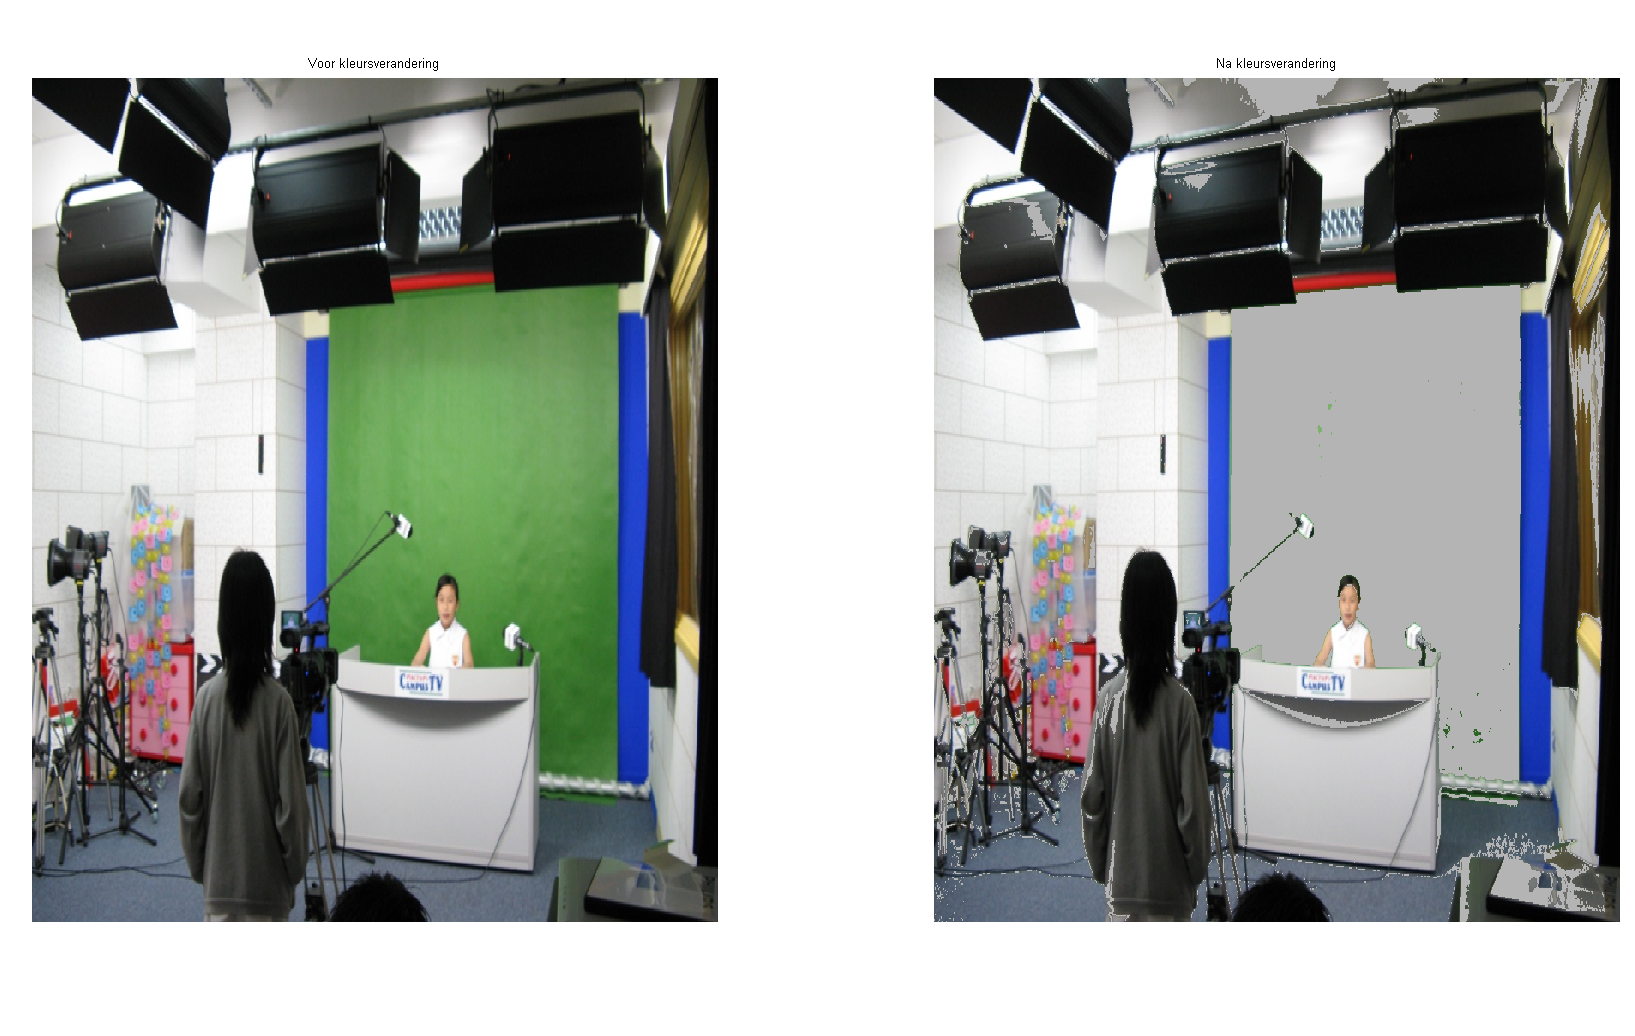
\includegraphics[width=0.95\textwidth]{Images/resultaat_chromakey.png}
				\caption{Resultaat achtergrond veranderen}
				\label{fig:achtergrond_veranderen}
				\end{figure}
		
		\par Uit bovenstaande figuur is af te leiden dat niet allen het groene scherm in de achtergrond veranderd is, maar ook enkele andere pixels in de achtergornd. Dit komt omdat
		er sommige stukken in de achtergrond nog een groene kleur bevat. Alles wat in het bereik van de groene kleur valt zal veranderd worden naar grijs.
		\noindent
		
		
		
		\subsection{Kleursverandering: uitbreiding}
		
		\subsubsection{Doelstelling}
			
			\par In de vorige opgave werd steeds iedere pixel in de afbeelding vergeleken om na te gaan of deze in het bereik valt van de groene kleur. Dit heeft als nadeel dat het 
			bereik experimenteel bepaald moet worden en vervolgens handmatig in de code dient ingesteld te worden. Met zou opteren voor een minder omslachtig proces dat minstens een 
			even goed resultaat aflevert. Wanneer men in een tv-studio gebruikt maakt van een groen scherm, wil men dit doorgaans niet gebruiken om het door \'e\'en andere kleur te 
			vervangen. Meestal gebruikt men dit om de achtergrond te veranderen. In deze uitbreiding zal ook geprobeerd worden om de groene achtergornd te veranderen naar een afbeelding
			met wolkjes. 
			
			\newpage 
		\subsubsection{Werkwijze en resultaat}
			
			\par De werkwijze is compleet verschillend met de werkwijze die gevolgd werd in bovenstaande opgaven. In de eerste plaats worden beide afbeeldingen ingeladen in de code. 
			vervolgens wordt ook al plaats gereserveerd om het eindresultaat in op te slaan. Vervolgens gaan we de kleurwaarden per pixel omzetten naar percentages. Dit wil zeggen dat
			we de rgb-waarden die vari\"eren van 0 tot 255 gaan delen door 255 zodat we het percentage bekomen, een getal tussen 0 en 1. \noindent \bigskip
			
			\par Vervolgens gaan we de groenwaarde van elke pixel. dit doen we door middel van de kleurkanalen met elkaar te vergelijken. Dit gebeurt aan de hand van volgende formule:
			groenwaarde = groen x (groen - rood) x (groen - blauw). Hierna wordt ook rekening gehouden met een bepaalde threshold, zodat we niet 1 tint groen bekijken, maar een aantal tinten
			groen die afgelijd zijn van het gemiddelde. Om na te gaan of een pixel groen is stellen we opnieuw een matrix op met daarin een 0 als de pixel niet groen is, en een 1 als de
			pixel wel groen is. De beslissing of een pixel al dan niet groen is wordt genomen op basis van de threshold. Wanneer de groenwaarde groter is dan de threshold, dan zal de pixel
			als groen bestempeld worden. \noindent \bigskip 
			
			\par Nu zullen voor elke kleur (R,G en B) de afbeeldingen overlopen worden. Per kleur zullen de pixels van het studiobeeld overschreven worden met die van de achtergrondafbeelding 
			indien er in de IsGroen matrix een 1 staat op de plaats met de overeenstemmende pixel. Het resultaat zal opgeslagen worden in een nieuwe variabale.
		    De Matlabcode die bij deze werkwijze hoort, wordt hieronder weergegeven:  \bigskip
			
			\lstinputlisting[caption=Matlab-code achtergrond veranderen]{Matlab/opgave_2_extra.m}
			
			\par Het resultaat van deze aanpak is te zien in volgende figuur:
			
				\begin{figure}[H]
				\centering
				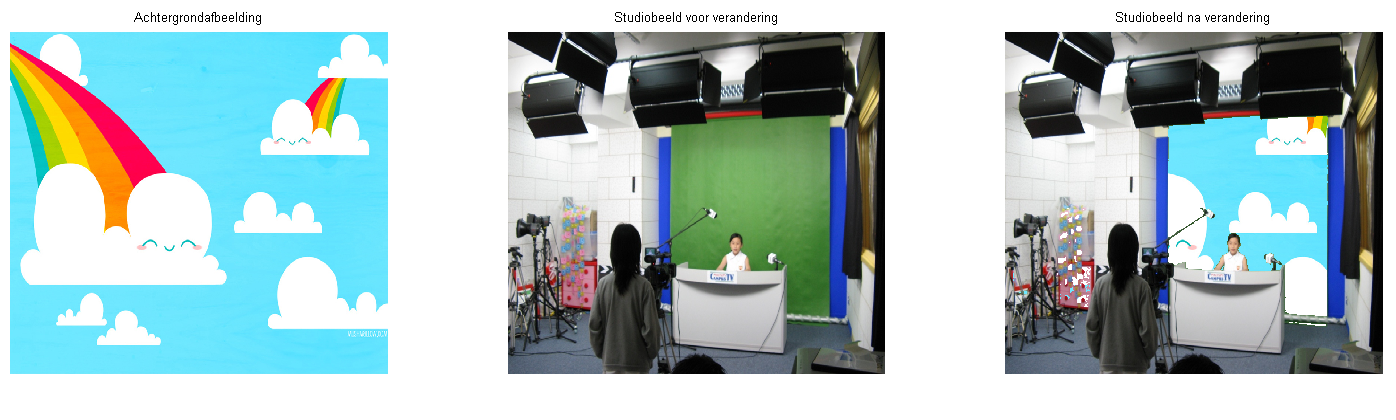
\includegraphics[width=0.95\textwidth]{Images/resultaat_chromakey_extra.png}
				\caption{Resultaat achtergrond veranderen - uitbreiding}
				\label{fig:resultaat_chromakey_extra}
				\end{figure}
				
			\par Men kan opmerken dat inderdaad de groene achtergrond veranderd is naar de wolkjes. Men dient wel op te merken dat beide afbeeldingen even groot moeten zijn om bovenstaande code
			correct te kunnen uitvoeren. De code is dus nog niet optimaal, maar maakt het wel al mogelijk de achtergrond te veranderen zonder dat er een kleurenbereik ingesteld dient te worden.
			
 \chapter{Algemeen besluit}
 
\par Na deze verschillende opdrachten uit te voeren, en zelf ook wat variaties op de oefeningen met Matlab geoefend te hebben is het begrip DSP op vlak van video toch heel wat opgeklaard.
We kunnen reeds een een verzameling aan kleuren binnen vooropgestelde rgb-grenzen vervangen door een andere kleur. Hoe nauwer deze grenzen, hoe minder de afbeelding zal worden be\"invloed. 
Als dit mogelijk is voor een enkel frame, rest ons enkel nog de stap naar real-time processing.
Dit houdt in dat er continue frames binnekomen die dan ook \'e\'en voor \'e\'en ver- en bewerkt moeten worden.
Als we elk zo'n frame als een enkele statische afbeelding kunnen bewerken, kunnen we de reeds opgedane ervaring inzetten om sneller tot ons gewenste resultaat te komen.
Indien de overstap van Matlab naar DSP++ niet te groot is, dan hebben we ons dus reeds voorbereid op de uiteindelijke opgave.


% Indien er bijlagen zijn:
\appendixpage*          % indien gewenst
\appendix
 \chapter{Matlab Code}
 \section{Opgave 1 Deel 1}
\lstinputlisting[caption=Matlab-code \'e\'erste aanpak]{Matlab/Smurf_1.m}
\newpage
 \section{Opgave 1 Deel 2}
\lstinputlisting[caption=Matlab-code tweede aanpak]{Matlab/Smurf_2.m}
\newpage
 \section{Opgave 2 Deel 1}
\lstinputlisting[caption=Matlab-code achtergrond veranderen]{Matlab/opgave_2_1.m}
\newpage
 \section{Opgave 2 Deel 2}
\lstinputlisting[caption=Matlab-code achtergrond veranderen]{Matlab/opgave_2_extra.m}


\backmatter


\end{document}


